% !TEX root = main.tex
\section{Nowa implementacja modułu AthenaMonitoring}
Głównym celem refaktoringu framworka, było oddzielenie kodu odpowiedzialnego za zarządzanie histogramami od kodu algorytmów. 
Dzięki takiemu rozgraniczeniu odpowiedzialności, twórcy algorytmów mogą skupić się na ich poprawnej implementacji i określeniu które wartości powinny znaleźć się na wykresach jako wynik. 
Natomiast to kiedy stworzyć histogram, jak go wypełnić i zapisać jest obsługiwane przez wspólny kod. 

Sercem nowego rozwiązania jest GenericMonitoringTool - nowe narzędzie w ramach frameworka Athena.
Zajmuje się on przygotowaniem histogramów i powiązaniem ich z kodem uruchamianych algorytmów. 
Działa on w oparciu o deklaracje.
Twórca algorytmu deklaruje zbiór wartości (obejmuje to skalary oraz tablice) jakie mogą być monitorowane w obrębie jego wykonania, oraz informuje GenericMonitoringTool kiedy są one gotowe do przekazania do histogramów.
Natomiast użytkownik takiego algorytmu, deklaruje jakie wykresy chciałby stworzyć i z użyciem których zmiennych. 
Następuje to w kroku konfiguracyjnym Athena Python, gdzie definiuje on typy histogramów, parametry binowania, zakresy wartości, opisy itd. 
Taki interfejs pozwala uniknąć rekompilacji kodu C++ za każdym razem, gdy użytkownik zmienia parametry wykresu. 

\begin{figure}[!ht]
\centering
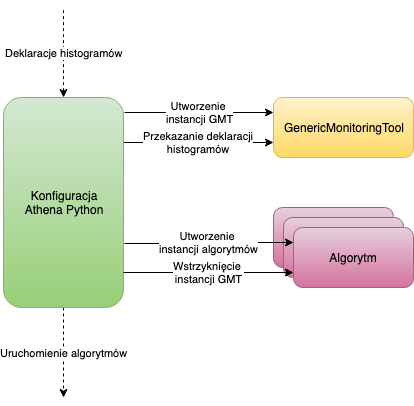
\includegraphics[width=0.75\textwidth]{img/algo_init.png}
\caption{
//TODO
}
\label{fig:athena:oldFlow}
\end{figure}

\begin{figure}[!ht]
\centering
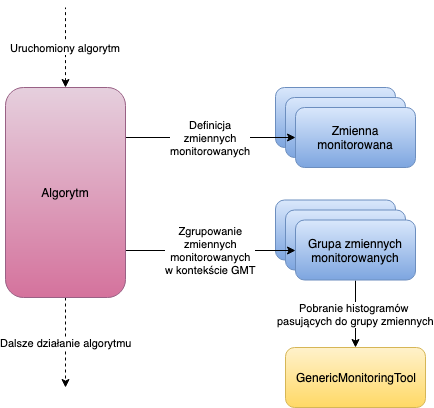
\includegraphics[width=0.75\textwidth]{img/algo_run.png}
\caption{
//TODO
}
\label{fig:athena:oldFlow}
\end{figure}

\subsection{Deklaracja histogramu}
"PATH, HTYPE, NAME, TITLE, BINNING, [LABELS], OPTIONS"

\subsection{Publiczny interfejs}

\subsubsection{GenericMonitoringTool}
Centralnym punktem nowej implementacji jest klasa GenericMonitoringTool, będąca narzędziem frameworka Athena.
Służy ona jako pomost pomiędzy konfiguracją napisaną w Pythonie, a kodem algorytmów w C++.
Jest zarządzana przez użytkownika i to do niej wstrzykuje się deklaracje histogramów jakie mają zostać utworzone podczas uruchomienia.
To ona odpowiada za przygotowanie i przechowywanie obiektów ROOT, wygenerowanych na podstawie tych deklaracji.
Dostęp do nich zapewnia poprzez warstwę abstrakcji zdefiniowaną w klasie HistogramFiller. 
Dodatkowo, posiada ona dostęp do aktualnych wartości Run Number i Lumi Block; dzięki temu możliwe jest generowanie grup histogramów w kontekście tych zmiennych. 
 
\subsubsection{HistogramDef}
Deklaracje histogramów na potrzeby GenericMonitoringTool reprezentowane są przez klasę HistogramDef.
To w niej zachodzi parsowanie ciągu znaków podanego przez użytkownika i wstępna weryfikacja jego poprawności.
Dzięki niej łatwiejszy jest dostęp do wybranych danych o histogramie. 
Jeśli parsowanie z jakiegoś powodu się nie powiedzie, użytkownik zostanie o tym poinformowany poprzez wyjątek, wraz z opisem problemu.

\subsubsection{IHistogramProvider}
Interfejs IHistogramProvider został przygotowany z myślą o zapewnieniu warstwy abstrakcji pomiędzy frameworkiem ROOT, a kodem do monitorowania zmiennych. 
Zawiera on jedną metodę - `histogram()`; to ona wykorzystywana jest, aby pobrać odpowiedni obiekt histogramu do wypełnienia.

\subsubsection{IMonitoredVariable}
Interfejs IMonitoredVariable stanowi bazę dla wszystkich zmiennych monitorowanych. 
Zawiera on nazwę zmiennej oraz metodę `getVectorRepresentation()`, która musi zostać zaimplementowana przez klasy pochodne.
Framework dostarcza gotowe implementacje tego interfejsu, jednak w specyficznych przypadkach użytkownik może sam go zaimplementować.  

\subsubsection{MonitoredScalar}
MonitoredScalar jest implementacją interfejsu IMonitoredVariable, reprezentującą pojedynczą wartość. 
Może ona być dowolnego typu, dopóki możliwe jest zrzutowanie go do `double`.
Definicja tej klasy pozwala wielokrotnie pobierać i modyfikować jej aktualną wartość.
Użytkownik może zdefiniować transformację tej zmiennej, która zostanie zaaplikowana w momencie pobrania jej wartości na potrzeby wypełnienia histogramu.

\subsubsection{MonitoredCollection}
MonitoredCollection jest implementacją interfejsu IMonitoredVariable, reprezentującą kolekcję wartości. 
Może ona być dowolnego typu, dopóki możliwe jest zrzutowanie wartości tej kolekcji do `double`.
Po utworzeniu obiektu tego typu, nie można go bezpośrednio modyfikować.
Jednak wszystkie zmiany przeprowadzone na kolekcji, zostaną odzwierciedlone w końcowym wyniku.
Użytkownik może zdefiniować transformację dla obiektów znajdujących się w kolekcji, która zostanie zaaplikowana w momencie pobrania ich wartości na potrzeby wypełnienia histogramu.

\subsubsection{MonitoredTimer}
MonitoredTimer jest implementacją interfejsu IMonitoredVariable, która pozwala mierzyć czas w mikrosekundach.
Dostarcza metody `start()` i `stop()`, zapewniające kontrole nad jej zachowaniem.
Wymagane jest, aby nazwy zmiennych tego typu posiadały prefix `TIME\_`.

\subsubsection{MonitoredGroup}
Miejscem w którym zmienne monitorowane kojarzone są z odpowiednimi histogramami jest klasa MonitoredGroup. 
Przyjmuje ona referencje do GenericMonitoringTool i zbioru IMonitoredVariable.
Na tej podstawie pobiera listę obiektów HistogramFiller, które są zapamiętywane w jej kontekście.
Dzięki temu możliwe jest określenie, kiedy i które histogramy należy wypełnić oraz jakie zmienne mają być użyte w tym celu.
Domyślnie wypełnienie następuje, gdy wywoływany jest destruktor obiektu MonitoredGroup. 
Jednakże, można to zrobić manualnie używając metody `fill()`.
Stworzenie obiektu MonitoredGroup jest niezbędne do używania zmiennych monitorowanych, ponieważ bez grupy, niemożliwe jest skojarzenie zmiennych z histogramami. 

\subsubsection{HistogramFiller}
Klasa abstrakcyjna HistogramFiller agreguje wszystkie dane niezbędne do poprawnego wypełnienia histogramów danymi. 
To ona przechowuje referencje do instancji IHistogramProvider, HistogramDef, zbioru IMonitoredVariable i mutexów.
Zapewnia interfejs do wypełniania histogramów w postaci metody `fill()`.
Klasy pochodne, powinny ją zaimplementować i wpisać dane ze zmiennych monitorowanych do histogramów ROOT.
W tej metodzie używany jest również mutex do zapewnienia spójności danych i synchronizacji pomiędzy różnymi wątkami. 

\subsubsection{HistogramDefParseException}
HistogramDefParseException reprezentuje błędy powstałe przy próbie sparsowania deklaracji histogramu dostarczonej przez użytkownika.
Zawiera on informacje o przyczynie problemu.

\subsubsection{HistogramException}
HistogramException reprezentuje błędy powstałe przy próbie utworzenia obiektów ROOT na podstawie HistogramDef.
Zawiera on informacje o przyczynie problemu.

\subsection{Niepubliczny interfejs}

\subsubsection{HistogramFactory}
Klasa HistogramFactory stanowi bezpośrednią warstwę komunikacji z serwisem THistSvc w którym tworzone są obiekty ROOT.
Odpowiada ona za interpretację HistogramDef, stworzenie histogramu odpowiedniego typu i skonfigurowanie go na podstawie tej deklaracji.
Dodatkowo zapewnia mechanizm ponownego użycia raz już stworzonych histogramów, co zwiększa wydajność tego rozwiązania.

\subsubsection{HistogramFillerFactory}
Głównym zadaniem klasy HistogramFillerFactory jest utworzenie odpowiedniego zestawu obiektów IHistogramProvider i HistogramFiller na podstawie dostarczonej definicji histogramu w kontekście GenericMonitoringTool.

\subsubsection{Implementacje IHistogramProvider}
\begin{itemize}
\item StaticHistogramProvider

	Charakteryzuje się tym, że obiekt histogramu jest tworzony i zapamiętywany w konstruktorze tego obiektu. Zapewnia to szybszy dostęp do histogramu przy jego wypełnianiu. 
\item LumiblockHistogramProvider

	Cechą charakterystyczną tej implementacji jest to, że zwraca ona różne obiekty histogramów na podstawie aktualnej wartości Lumi Block. 
	Na to jaka instancja zostanie zwrócona, wpływa parametr kLBNHistoryDepth.
	Określa on, jak liczne są grupy w które łączone są wyniki.
	Te dwie informacje pozwalają zdecydować do której grupy ma trafić aktualna wartość.
	Konsekwencją takiej funkcjonalności jest konieczność każdorazowego odwoływania się do THistSvc po odpowiedni obiekt ROOT, co nieco spowalnia wypełnianie tego typu histogramów.
\item OfflineHistogramProvider

	Cechuje się tym, że to jaki obiekt histogramu zostanie zwrócony, wpływają aktualne wartości: Lumi Block, Run Number oraz konwencja histogramu.
	Jest przeznaczony dla uruchomień typu Offline.
	Podobnie jak dla LumiblockHistogramProvider, konieczne jest każdorazowe odwołanie się do THistSvc, w celu pobrania odpowiedniej instancji ROOT.
\end{itemize}

\subsubsection{Implementacje HistogramFiller}
Wszystkie poniższe implementacje, używają mutexa dostarczonego przez klasę bazową do synchronizacji wątków. 
\begin{itemize}
\item HistogramFiller1D

	Jest to domyślna klasa odpowiadająca za wypełnianie wszystkich typów histogramów jednowymiarowych TH1. 
\item CumulativeHistogramFiller1D

	Ta implementacja jest używana, gdy użytkownik zadeklaruje histogram z opcją `kCumulative`.
	Cechuje się tym, że dodawana jest wartość 1 do wszystkich binów histogramu o indeksach mniejszych lub równych indeksowi binu do którego należałoby dodać aktualnie przetwarzaną wartość.
\item HistogramFillerRebinable1D

	Ta implementacja jest używana, gdy użytkownik zadeklaruje histogram z opcją `kAddBinsDynamically`.
	Jej cechą szczególną jest automatyczne zwiększanie zakresu danych histogramu, gdy nowa wartość jest spoza tego zakresu. Za każdym razem jest on zwiększany dwukrotnie do momentu, aż nowa wartość zawierać się będzie w nowym zakresie.
\item VecHistogramFiller1D

	Ta implementacja jest używana, gdy użytkownik zadeklaruje histogram z opcją `kVec`.
	Jest ona przeznaczona głownie do zmiennych typu MonitoredCollection.
	Iteruje po wszystkich wartościach z kolekcji i przepisuje ich wartości do binów o indeksach odpowiadających indeksom z tej kolekcji.
\item VecHistogramFiller1DWithOverflows

	Ta implementacja jest używana, gdy użytkownik zadeklaruje histogram z opcją `kVecUO`.
	Działa bardzo podobnie do VecHistogramFiller1D, z tą różnicą, że nie zabezpiecza użytkownika przed przepełnieniem histogramu.
\item HistogramFiller2D

	Jest to domyślna klasa odpowiadająca za wypełnianie wszystkich typów histogramów dwuwymiarowych TH2.
	Do wypełnienia histogramu wykorzystuje ona dwie zmienne monitorowane jednocześnie.
	Aby ten proces przebiegł poprawnie, reprezentacje tych zmiennych muszą być równolicznymi kolekcjami lub jedna z nich musi zawierać dokładnie jeden element. 
\item HistogramFillerProfile

	Ta implementacja jest używana, gdy użytkownik zadeklaruje histogram typu `TProfile`.
	Wypełnienie przebiega tak samo jak dla HistogramFiller2D.
\item HistogramFiller2DProfile

	Ta implementacja jest używana, gdy użytkownik zadeklaruje histogram typu `TProfile2D`.
	Do wypełnienia histogramu wykorzystuje ona trzy zmienne monitorowane jednocześnie.
	Aby ten proces przebiegł poprawnie, reprezentacje tych zmiennych muszą być równolicznymi kolekcjami.
\item HistogramFillerEfficiency

	Ta implementacja jest używana, gdy użytkownik zadeklaruje histogram typu `TEfficiency`.
	Do wypełnienia histogramu wykorzystuje ona dwie zmienne monitorowane jednocześnie.
	Aby ten proces przebiegł poprawnie, reprezentacje tych zmiennych muszą być równolicznymi kolekcjami.
	
\end{itemize}